\newpage
\section{Documento dei Requisiti}

\subsection{Raccolta dei requisiti}

\begin{itemize}
  \item[-] I clienti delle farmacie hanno a disposizione due servizi: controllare se un farmaco è disponibile vicino alla loro posizione e/o prenotarlo.
  \item[-] Il cliente fornisce la sua posizione che l'applicativo userà per indicargli le farmacie più vicine. Contemporaneamente specificherà il farmaco da cercare e l'applicativo fornirà le 10 farmacie più vicine ad averlo in magazzino indicando se è disponibile o se sta per terminare.
  \item[-] Per la prenotazione è necessario possedere un account
  \item[-] La prenotazione sarà composta da uno o più farmaci, dalla farmacia, e dal giorno. 
  \item[-] L'account viene creato in due fasi:\\
      1. Registrazione con nome, cognome, password, data di nascita, email e codice fiscale\\
      2. Autenticazione di persona in farmacia
  \item[-] La email deve essere univoca, la password di almeno 8 caratteri, contentente almeno un numero e un carattere alfabetico.
  \item[-] Per l'autenticazione è necessario mostrare il tesserino sanitario per l'identificazione in farmacia.
  \item[-] Il cliente può vedere la lista delle sue prenotazioni in corso
  \item[-] Il farmacista vede le prenotazioni, i farmaci disponibili in negozio e viene segnalato riguardo ai farmaci in esaurimento
  \item[-] Il farmacista può confermare le prenotazioni andate a buon fine
  \item[-] Se alla fine della giornata un utente non si presenta allora l'evento viene registrato, per poi avvisare il farmacista che può eventualmente bloccare l'utente
  \item[-] Il sistema sarà ovviamente distribuito e di natura client-server con la presenza di un database centrale dove memorizzare i dati
  \item[-] La gestione delle vendite, degli ordini e modifiche di magazzino è gestita da un altro software
  \item[-] Non va considerata la gestione dei dati del personale 
\end{itemize}


\subsection{Tabella dei Requisiti}

\begin{tabular} {|P{1.5cm}|P{12.5cm}|P{3cm}|}
\hline
  \textbf{ID} & \textbf{Requisiti} & \textbf{Tipo} \\
\hline
  R1F & Localizzazione delle farmacie più vicine in base al farmaco da cercare & Funzionale \\
\hline
  R2F & Specifica del farmaco da cercare da parte dell'utente & Funzionale \\
\hline
  R3F & Presentazione delle farmacie che dispongono di un farmaco & Funzionale \\
\hline 
  R4F & Registrazione di un account tramite l'interfaccia web & Funzionale\\
\hline
  R5F & Attivazione dell'account con identificazione fisica dell'utente con documento & Funzionale \\
\hline
  R6F & La prenotazione sarà composta da uno o più farmaci, dalla farmacia e dal giorno & Funzionale\\
\hline
  R7F & Identificazione attraverso email univoca e password di almeno 8 caratteri, contentente almeno un carattere alfabetico e un carattere numerico & Funzionale\\
\hline
  R8F & Visualizzazione delle prenotazioni del cliente & Funzionale\\
\hline
  R9F & Visualizzazione delle prenotazioni della farmacia & Funzionale\\
\hline
  R10F & Visualizzazione del numero dei farmaci disponibili & Funzionale\\
\hline
  R11F & Notifica dei farmaci in esaurimento o in scadenza & Funzionale\\
\hline
  R12F & Conferma della prenotazione andata a buon fine & Funzionale\\
\hline
  R13F & Notifica della mancata finzalizzazione in acquisto di una prenotazione & Funzionale\\
\hline
  R14F & Blocco dell'utente che effettua troppe prenotazioni senza presentarsi & Funzionale\\
\hline
  R15F & Verrà memorizzato il numero di prenotazioni andate a buon fine & Funzionale\\
\hline
  R1NF & Velocità di memorizzazione dei dati & Non Funzionale\\
\hline
  R2NF & Velocità della ricerca dei dati & Non Funzionale\\
\hline
  R3NF & Semplicità dell'interfaccia & Non Funzionale\\
\hline
  R4NF & Un utente non può avere più di un account verificato & Non Funzionale\\
\hline
  R5NF & la gestione delle vendite e ordini è gestita da un altro software & Non Funzionale\\
\hline
  R6NF & Per prenotare l'utente deve essere registrato & Non Funzionale\\
\hline
  R7NF & La gestione delle vendite, degli ordini e modifiche di magazzino è gestita da un altro software & Non Funzionale\\
\hline
  R8NF & Non va considerata la gestione dei dati del personale & Non Funzionale \\
\hline
\end{tabular}

\subsection{Analisi dei Requisiti}
\subsubsection{Vocabolario}

\begin{tabular} {|P{3.5cm}|P{10.5cm}|P{3cm}|}
\hline
  \textbf{Voce} & \textbf{Definizione} & \textbf{Sinonimi}\\
\hline
  Cliente & Persona che usufruisce del servizio lato cliente & Utente \\
\hline
  ClienteRegistrato & Cliente che possiede un account identificato con cui può effettuare prenotazioni & UtenteRegistrato \\
\hline
  Farmacia & Farmacia che aderisce al servizio & Punto vendita\\
\hline
  Farmaco & Medicinale che viene venduto in farmacia & \\
\hline
  Farmacista & Utente che accede con le credenziali della farmacia & Operatore \\
\hline
  Prenotazione & Richiesta di farmaci da comprare in negozio & \\
\hline
  Data e ora prenotazione & Indicazione temporale del momento in cui avverrà la prenotazione & \\
\hline
  Posizione & Luogo della ricerca o collocamento geografico della farmacia & \\
\hline
  Credenziali & Insieme composto da email e password necessari per accedere al sistema&\\
\hline
  Email & Indirizzo di posta elettronica del cliente utilizzata anche per l'autenticazione &\\
\hline
  Password & Codice alfanumerico di almeno 8 caratteri &\\
\hline
  Magazzino & Luogo fisico in cui vengono conservati i farmaci di un punto vendita & Deposito \\
\hline
\end{tabular}

\subsubsection{Sistemi esterni}

Il sistema dovrà interfacciarsi con un sistema esterno il quale si occupa di
mantenere una lista aggiornata dei farmaci in magazzino e degli
acquisti avvenuti in ogni farmacia associata.


\newpage %optional
\subsubsection{Casi d'uso della farmacia}

\begin{figure}[h!]
  \begin{center}
      \includegraphics[width=\textwidth]{casiUso.jpg}
  \end{center}
\end{figure}

\newpage %optional
\subsubsection{Scenari}
\hfill \break

%GestioneFarmacia
\begin{tabular} {|P{4.5cm}|P{12.5cm}|}
\hline  
  \textbf{Titolo} & GestioneFarmacia \\
\hline
  \textbf{Descrizione} & Gestione dell'utenza di un cliente registrato \\
\hline
  \textbf{Attori} & Farmacista\\
\hline
  \textbf{Relazioni} & Login, SospensioneUtenza, ControlloUtenti, ResocontoFarmaci, ControlloPrenotazioni\\
\hline
  \textbf{Precondizioni} & \\
\hline
  \textbf{Postcondizioni} & \\
\hline
  \textbf{Scenario Principale} & 1. Login \\ 2. Il farmacista può eseguire la verifica, sospendere un account, controllare le prenotazioni \\
\hline
  \textbf{Scenari Alternativi} &\\
\hline
  \textbf{Requisiti non funzionali} & Velocità di ricerca dei dati e semplicità di navigazione tra le diverse maschere\\
\hline
  \textbf{Punti aperti} &\\
\hline
\end{tabular}
\hfill
\break

%ResocontoFarmaci
\begin{tabular} {|P{4.5cm}|P{12.5cm}|}
  \hline
    \textbf{Titolo} & ResocontoFarmaci\\
  \hline
    \textbf{Descrizione} & Viene mostrato l'elenco dei farmaci in scadenza o in esaurimento\\
  \hline
    \textbf{Attori} & Farmacista\\
  \hline
    \textbf{Relazioni} & GestioneFarmacia\\
  \hline
    \textbf{Precondizioni} &\\
  \hline
    \textbf{Postcondizioni} & Viene mostrato l'elenco degli Utenti a rischio sospensione\\
  \hline
    \textbf{Scenario Principale} & 1. Il Farmacista va nella schermata di visualizzazione farmaci \\ 2. Il sistema recupera l'elenco dei farmaci in esaurimento o in scadenza \\ 3. Il sistema mostra a video l'elenco richiesto\\
  \hline
    \textbf{Scenari Alternativi} &\\
  \hline
    \textbf{Requisiti non funzionali} & Velocità di ricerca dei dati e semplicità di navigazione tra le diverse maschere\\
  \hline
    \textbf{Punti aperti} &\\
  \hline
\end{tabular}
\hfill
\break

%ControlloUtenti
\begin{tabular} {|P{4.5cm}|P{12.5cm}|}
\hline
  \textbf{Titolo} & ControlloUtenti\\
\hline
  \textbf{Descrizione} & Si controllano gli utenti con potenzialmente sospendibili\\
\hline
  \textbf{Attori} & Farmacista\\
\hline
  \textbf{Relazioni} & SospensioneUtenza, GestioneFarmacia\\
\hline
  \textbf{Precondizioni} &\\
\hline
  \textbf{Postcondizioni} & Viene mostrato l'elenco degli Utenti a rischio sospensione\\
\hline
  \textbf{Scenario Principale} & 1. Il Farmacista va nella schermata di visualizzazione utenti \\ 2. Il sistema recupera l'elenco degli utenti a rischio o sospesi \\ 3. Il sistema mostra a video l'elenco degli utenti\\
\hline
  \textbf{Scenari Alternativi} &\\
\hline
  \textbf{Requisiti non funzionali} & Velocità di ricerca dei dati e semplicità di navigazione tra le diverse maschere\\
\hline
  \textbf{Punti aperti} & \\
\hline
\end{tabular}
\hfill
\break

%SospensioneUtenza
\begin{tabular} {|P{4.5cm}|P{12.5cm}|}
  \hline
    \textbf{Titolo} & SospensioneUtenza\\
  \hline
    \textbf{Descrizione} & Se un utente non ha concluso troppe prenotazioni allora viene proposta la sospensione dell'utente al farmacista\\
  \hline
    \textbf{Attori} & Farmacista\\
  \hline
    \textbf{Relazioni} & ControlloPrenotazioni, GestioneFarmacia\\
  \hline
    \textbf{Precondizioni} & Il cliente è diffidato dal sistema (ha molte prenotazioni non concluse)\\
  \hline
    \textbf{Postcondizioni} & Il cliente non può più effettuare prenotazioni per 30 giorni\\
  \hline
    \textbf{Scenario principale} & 1. ControlloUtenti \\ 2. Il farmacista può sospendere o annullare la sospensione di un utente \\
  \hline
    \textbf{Scenari alternativi} &\\
  \hline
    \textbf{Requisiti non funzionali} & Velocità nella ricerca dei dati e semplicità dell'interfaccia\\
  \hline
    \textbf{Punti aperti} &\\
  \hline
\end{tabular}
\hfill
\break

%ControlloPrenotazioni
\begin{tabular} {|P{4.5cm}|P{12.5cm}|}
\hline
  \textbf{Titolo} & ControlloPrenotazioni\\
\hline
  \textbf{Descrizione} & Si controllano le prenotazioni non terminate\\
\hline
  \textbf{Attori} & Farmacista\\
\hline
  \textbf{Relazioni} & ConfermaPrenotazione,GestioneFarmacia\\
\hline
  \textbf{Precondizioni} &\\
\hline
  \textbf{Postcondizioni} & Viene mostrato l'elenco delle prenotazioni\\
\hline
  \textbf{Scenario principale} & 1. Il Farmacista va nella schermata di visualizzazione prenotazioni \\ 2. Il sistema recupera l'elenco delle prenotazioni giornaliere \\ 3. Il sistema mostra a video l'elenco delle prenotazioni\\
\hline
  \textbf{Scenari Alternativi} &\\
\hline
  \textbf{Requisiti non funzionali} & Velocità di ricerca dei dati\\
\hline
  \textbf{Punti aperti} &\\
\hline
\end{tabular}
\hfill
\break

%ConfermaPrenotazione
\begin{tabular} {|P{4.5cm}|P{12.5cm}|}
\hline
  \textbf{Titolo} & ConfermaPrenotazione\\
\hline
  \textbf{Descrizione} & Il Farmacista conferma la prenotazione avvenuta\\
\hline
  \textbf{Attori} & Farmacista\\
\hline
  \textbf{Relazioni} & ControlloPrenotazioni\\
\hline
  \textbf{Precondizioni} &\\
\hline
  \textbf{Postcondizioni} & La prenotazione viene confermata\\
\hline
  \textbf{Scenario principale} & 1. ControlloPrenotazioni \\ 2. Il Farmacista conferma l'avvenuta prenotazione\\
\hline
  \textbf{Scenari Alternativi} & \\
\hline
  \textbf{Requisiti non funzionali} & Semplicità dell'interfaccia\\
\hline
  \textbf{Punti aperti} &\\
\hline
\end{tabular}
\hfill
\break

%VerificaIdentità
\begin{tabular} {|P{4.5cm}|P{12.5cm}|}
  \hline
    \textbf{Titolo} & VerificaIdentità\\
  \hline
    \textbf{Descrizione} & Verifica dell'identità dell'utente registrato\\
  \hline
    \textbf{Attori} & Cliente, Farmacista\\
  \hline
    \textbf{Relazioni} & GestioneFarmacia\\
  \hline
    \textbf{Precondizioni} & Il cliente è registrato\\
  \hline
    \textbf{Postcondizioni} & L'utente è stato verificato e il suo account viene abilitato per effettuare delle prenotazioni\\
  \hline
    \textbf{Scenario principale} & 1. Il cliente va in farmacia con il documento specificato in fase di registrazione \\ 2. Il cliente viene identificato dal farmacista \\ 3. Il farmacista chiede al sistema di recuperare l'utente \\ 4. Il farmacista attiva l'account dell'utente\\
  \hline
    \textbf{Scenari alternativi} & 4. Il sistema non trova nessun utente, segnala il farmacista\\
  \hline
  \textbf{Requisiti non funzionali} & Velocità di memorizzazione e semplicità di navigazione tra le diverse maschere\\
  \hline
    \textbf{Punti aperti} &\\
  \hline
\end{tabular}
\hfill
\break

%RicercaFarmaci
\begin{tabular} {|P{4.5cm}|P{12.5cm}|}
  \hline
    \textbf{Titolo} & RicercaFarmaci\\
  \hline
    \textbf{Descrizione} & L'utente verifica la disponibilità di un particolare farmaco nelle farmacie più vicine a lui\\
  \hline
    \textbf{Attori} & Cliente\\
  \hline
    \textbf{Relazioni} &\\
  \hline
    \textbf{Precondizioni} &\\
  \hline
    \textbf{Postcondizioni} & Si visualizza la lista delle farmacie con disponibilità\\
  \hline
    \textbf{Scenario principale} & 
      1. Il cliente si reca nella pagina di ricerca \\
      2. Il cliente inserisce il nome del farmaco per cui eseguire la ricerca \\
      3. Il sistema ottiene la lista delle farmacie aventi il farmaco specificato entro un range dalla località specificata. \\ 
      4. Il sistema ordina la lista in base alla distanza geografica dalla zona dell'utente, in ordine crescente \\
      5. La lista viene mostrata all'utente\\
  \hline
    \textbf{Scenari Alternativi} &
      Scenario alternativo A: \\
        1. Login \\ 
        2. Il cliente si reca nella pagina di ricerca \\ 
        3. Il cliente inserisce il nome del farmaco per cui eseguire la ricerca \\ 
        4. Il sistema ottiene la lista delle farmacie aventi il farmaco specificato entro un range dalla località specificata. \\ 
        5. Il sistema ordina la lista in base alla distanza geografica dalla zona dell'utente, in ordine crescente \\ 
        6. La lista viene mostrata all'utente \\ 
        7. L'utente può selezionare il farmaco per cominciare una prenotazione di quel farmaco nella farmacia scelta \\
      Scenario alternativo B: \\
        1. NuovaPrenotazione scenario alternativo A \\ 
        2. Il cliente inserisce il nome del farmaco per cui eseguire la ricerca \\ 
        3. Il sistema ottiene la lista dei farmaci disponibili nella farmacia scelta il cui nome inizia per il testo inserito dall'utente \\ 
        4. La lista viene mostrata all'utente \\ 
        5. L'utente può selezionare il farmaco corrispondente, se è presente nella lista, ed aggiungerlo alla prenotazione in corso \\
  \hline
    \textbf{Requisiti non funzionali} & Velocità di ricerca dei dati e semplicità di navigazione tra le diverse maschere\\
  \hline
    \textbf{Punti aperti} &\\
  \hline
\end{tabular}
\hfill
\break

%GestionePrenotazioni
\begin{tabular} {|P{4.5cm}|P{12.5cm}|}\hline
  \textbf{Titolo} & GestionePrenotazioni\\
  \hline
    \textbf{Descrizione} & Gestione delle prenotazioni di un cliente registrato\\
  \hline
    \textbf{Attori} & ClienteRegistrato\\
  \hline
    \textbf{Relazioni} & Login, ListaPrenotazioni, NuovaPrenotazione\\
  \hline
    \textbf{Precondizioni} &\\
  \hline
    \textbf{Postcondizioni} &\\
  \hline
    \textbf{Scenario Principale} & 1. Il cliente esegue il login \\ 2. Il cliente può visualizzare le proprie prenotazioni passate o in corso e può effettuare nuove prenotazioni.\\
  \hline
    \textbf{Scenari Alternativi} &\\
  \hline
    \textbf{Requisiti non funzionali} & Velocità di verifica dei dati e semplicità di navigazione tra le diverse maschere\\
  \hline
    \textbf{Punti aperti} &\\
  \hline
\end{tabular}
\hfill
\break

%NuovaPrenotazione
\begin{tabular} {|P{4.5cm}|P{12.5cm}|}
\hline
  \textbf{Titolo} & NuovaPrenotazione\\
\hline
  \textbf{Descrizione} & L'utente prenota a suo nome una lista di farmaci\\
\hline
  \textbf{Attori} & ClienteRegistrato\\
\hline
  \textbf{Relazioni} & GestionePrenotazioni\\
\hline
  \textbf{Precondizioni} &\\
\hline
  \textbf{Postcondizioni} & Il sistema ha memorizzato i dati della prenotazione, in attesa di conferma da parte della farmacia\\
\hline
  \textbf{Scenario principale} &
    1. RicercaFarmaci scenario alternativo A \\
    2. Il cliente può selezionare altri farmaci che vuole prenotare, la quantità, e inserisce la data di ritiro desiderata \\
    3. Il cliente invia la richiesta di prenotazione \\
    4. Il sistema pone la richiesta in attesa di conferma\\
\hline
  \textbf{Scenari Alternativi} & 
    Scenario A:
      1. Login \\
      2. Il cliente seleziona l'opzione "nuova prenotazione" \\
      3. Il cliente seleziona la farmacia e inserisce la data di ritiro desiderata \\
      4. Il cliente seleziona i farmaci che vuole prenotare e le relative quantità\\
      5. Il cliente invia la richiesta di prenotazione \\
      6. Il sistema pone la richiesta in attesa di conferma\\
    Scenario B: La farmacia non dispone dei farmaci richiesti. \\ 
    1. Il sistema nota che la farmacia non ha disponibilità di almeno uno dei farmaci specificati \\ 
    5. Viene inviato al cliente un messaggio di errore\\
\hline
  \textbf{Requisiti non funzionali} & Velocità di verifica dei dati e semplicità di navigazione tra le diverse maschere\\
\hline
  \textbf{Punti aperti} &\\
\hline
\end{tabular}
\hfill
\break

%ListaPrenotazioni
\begin{tabular} {|P{4.5cm}|P{12.5cm}|}
\hline
  \textbf{Titolo} & ListaPrenotazioni\\
\hline
  \textbf{Descrizione} & L'utente ottiene la lista delle proprie prenotazioni passate ed in corso\\
\hline
 \textbf{Attori} & ClienteRegistrato\\
\hline
  \textbf{Relazioni} & GestionePrenotazioni\\
\hline
  \textbf{Precondizioni} &\\
\hline
  \textbf{Postcondizioni} & Al cliente viene mostrata la lista delle prenotazioni passate ed in corso\\
\hline
  \textbf{Scenario Principale} & 1. Login \\ 2. Il cliente seleziona l'opzione di visualizzazione della lista delle prenotazioni \\ 3. Al cliente viene mostrato l'elenco delle prenotazioni effettuate\\
\hline
  \textbf{Scenari Alternativi} &\\
\hline
  \textbf{Requisiti non funzionali} & Velocità di verifica dei dati e semplicità di navigazione tra le diverse maschere\\
\hline
  \textbf{Punti aperti} &\\
\hline
\end{tabular}
\hfill
\break

%Login
\begin{tabular} {|P{4.5cm}|P{12.5cm}|}
\hline
  \textbf{Titolo} & Login\\
\hline
  \textbf{Descrizione} & Permette di accedere al sistema\\
\hline
  \textbf{Attori} & ClienteRegistrato, Farmacista\\
\hline
  \textbf{Relazioni} & NuovaPrenotazione, GestioneFarmacia\\
\hline
  \textbf{Precondizioni} &\\
\hline
  \textbf{Postcondizioni} & L'utente ha accesso al sistema, limitato in base ai suoi privilegi\\
\hline
  \textbf{Scenario principale} & 1. L'utente inserisce le credenziali di accesso \\ 2. Il sistema verifica le credenziali \\ 3. Se le credenziali sono corrette, viene presentata la schermata iniziale\\
\hline
  \textbf{Scenari Alternativi} & Scenario a: Credenziali non riconosciute. \\ 3. Il sistema non riconosce le credenziali e rispedisce l'utente alla schermata di login con un messaggio di errore\\
\hline
  \textbf{Requisiti non funzionali} & Velocità di verifica delle credenziali\\
\hline
  \textbf{Punti aperti} &\\
\hline
\end{tabular}
\hfill
\break

%Registazione
\begin{tabular} {|P{4.5cm}|P{12.5cm}|}
  \hline
    \textbf{Titolo} & Registrazione\\
  \hline
    \textbf{Descrizione} & Il cliente si registra al servizio\\
  \hline
    \textbf{Attori} & Cliente\\
  \hline
    \textbf{Relazioni} &\\
  \hline
  \textbf{Precondizioni} & Il cliente dispone di un codice fiscale valido\\
  \hline
    \textbf{Postcondizioni} & Il cliente è registrato nel sistema ed è posto in attesa della verifica\\
  \hline
    \textbf{Scenario principale} & 1. Il cliente accede alla sezione di registrazione \\ 2. Il cliente inserisce i propri dati: nome, cognome, data di nascita, email, password e il codice fiscale \\ 3. Il cliente termina la registrazione, se avvenuta con successo gli viene mostrata la conferma e viene reindirizzato alla pagina principale\\
  \hline
    \textbf{Scenari Alternativi} & Scenario a: il codice fiscale è già registrato \\ 3. Il sistema verifica che è già presente un utente con quel codice fiscale, quindi notifica il cliente con un messaggio di errore.\\
  \hline
    \textbf{Requisiti non funzionali} & Semplicità dell'interfaccia\\
  \hline
    \textbf{Punti aperti} &\\
  \hline
\end{tabular}
\hfill
\break

%AggiornamentoUtenti
\begin{tabular} {|P{4.5cm}|P{12.5cm}|}
\hline
  \textbf{Titolo} & AggiornamentoUtenti\\
\hline
  \textbf{Descrizione} & Aggiorna l'elenco degli utenti a rischio sospensione\\
\hline
  \textbf{Attori} & FineGiornata\\
\hline
  \textbf{Relazioni} &\\
\hline
  \textbf{Precondizioni} &\\
\hline
  \textbf{Postcondizioni} & Il DataBase degli utenti è aggiornato\\
\hline
  \textbf{Scenario principale} & 1. Si verifica l'evento FineGiornata\\ 2. Il sistema controlla le prenotazioni non andate a buon fine \\ 3. Il sistema aggiorna i dati relativi alle infrazioni degli utenti\\
\hline
  \textbf{Scenari Alternativi} &\\
\hline
  \textbf{Requisiti non funzionali} & Velocità della ricerca dei dati\\
\hline
  \textbf{Punti aperti} &\\
\hline
\end{tabular}
\hfill
\break

%AggiornamentoFarmaci
\begin{tabular} {|P{4.5cm}|P{12.5cm}|}
\hline
  \textbf{Titolo} & Aggiornamento Farmaci\\
\hline
  \textbf{Descrizione} & Aggiorna l'elenco dei farmaci in magazzino\\
\hline
  \textbf{Attori} & ModificheFarmaci\\
\hline
  \textbf{Relazioni} &\\
\hline
  \textbf{Precondizioni} &\\
\hline
  \textbf{Postcondizioni} & Il DataBase dei farmaci è aggiornato\\
\hline
  \textbf{Scenario principale} & 1. Si verifica l'evento ModificheFarmaci \\ 2. Il sistema recupera le modifiche dal DataBase Remoto \\ 3. Il sistema aggiorna i dati relativi ai farmaci in magazzino\\
\hline
  \textbf{Scenari Alternativi} &\\
\hline
  \textbf{Requisiti non funzionali} & Velocità della ricerca dei dati\\
\hline
  \textbf{Punti aperti} &\\
\hline
\end{tabular}
\hfill
\break

\subsection{Analisi del Rischio}

\subsubsection{Tabella Valutazione dei Beni}

\begin{tabular} {|P{4cm}|P{6cm}|P{7cm}|}
\hline
  \textbf{Bene} & \textbf{Valore} & \textbf{Esposizione}\\
\hline
  Sistema Informativo & Alto. Fondamentale per il funzionamento del servizio & Alta. Perdita finanziaria e di immagine\\
\hline
  Informazioni dei clienti & Alto. Dati generali dei clienti della farmacia, comprese le credenziali & Alta. Perdita di immagine dovuta alla divulgazione di dati sensibili\\
\hline
  Informazioni relative al personale & Alto. Dati relativi ai farmacisti, incluse le credenziali di accesso all'area riservata & Molto Alta. Perdita finanziaria dovuta a usi impropri delle credenziali con privilegi elevati. Perdita di immagine possibile con la divulgazione dei dati relativi ai clienti\\
\hline
  Dati delle prenotazioni & Alto. Necessario per tenere traccia delle prenotazioni & Molto Alta. Perdita finanziaria dovuta allo smarrimento di prenotazioni. Perdita di immagine con la divulgazione dei farmaci prenotati dai clienti\\
\hline
\end{tabular}

\subsubsection{Tabella Minacce/Controlli}

\begin{tabular} {|P{3.5cm}|P{2.5cm}|P{6cm}|P{5cm}|}
\hline
  \textbf{Minaccia} & \textbf{Probabilità} & \textbf{Controllo} & \textbf{Fattibilità}\\
\hline
  Furto credenziali Farmacista & Alta & Controllo sulla sicurezza della password - Log delle operazioni & Costo implementativo molto basso\\
\hline
  Furto credenziali Cliente & Alta & Controllo sulla sicurezza della password - Log delle operazioni & Costo implementativo molto basso\\
\hline
  Alterazione o intercettazione delle comunicazioni & Alta & Utilizzo di un canale sicuro - Log delle operazioni & Basso costo di realizzazione con determinati protocolli\\
\hline
  Accesso non autorizzato al database & Bassa & Accesso da macchine sicure - Log di tutte le operazioni & Basso costo di realizzazione, il server deve essere ben custodito\\
\hline
  DoS & Bassa & Controllo e limitazione delle richieste & Media complessità di implementazione\\
\hline
  Saturazione del database & Bassa & 1. Limitazione delle richieste in un dato intervallo di tempo. 2. Limite di tempo per la verifica di un cliente & Media complessità di implementazione\\
\hline
\end{tabular}

\subsubsection{Analisi Tecnologica della Sicurezza}

\begin{tabular} {|P{4cm}|P{13cm}|}
\hline
  Tecnologia & Vulnerabilità\\
\hline
  Autenticazione email/password & • Utente rivela volontariamente la password Utente rivela la password con un attacco di ingegneria sociale \\ • Utente non esce dal sistema dopo aver eseguito le operazioni \\ • Password banali\\
\hline
  Cifratura comunicazioni & • In caso di cifratura simmetrica particolare attenzione va alla lunghezza delle chiavi ed alla loro memorizzazione \\ • La memorizzazione è un fattore fondamentale anche nella cifratura asimmetrica\\
\hline
  Architettura Client/Server & • DoS \\ • Man in the Middle \\ • Sniffing delle comunicazioni\\
\hline
\end{tabular}

\newpage
\subsubsection{Security Use Case \& Misuse Case}
\par

\begin{figure}[h!]
  \begin{center}
      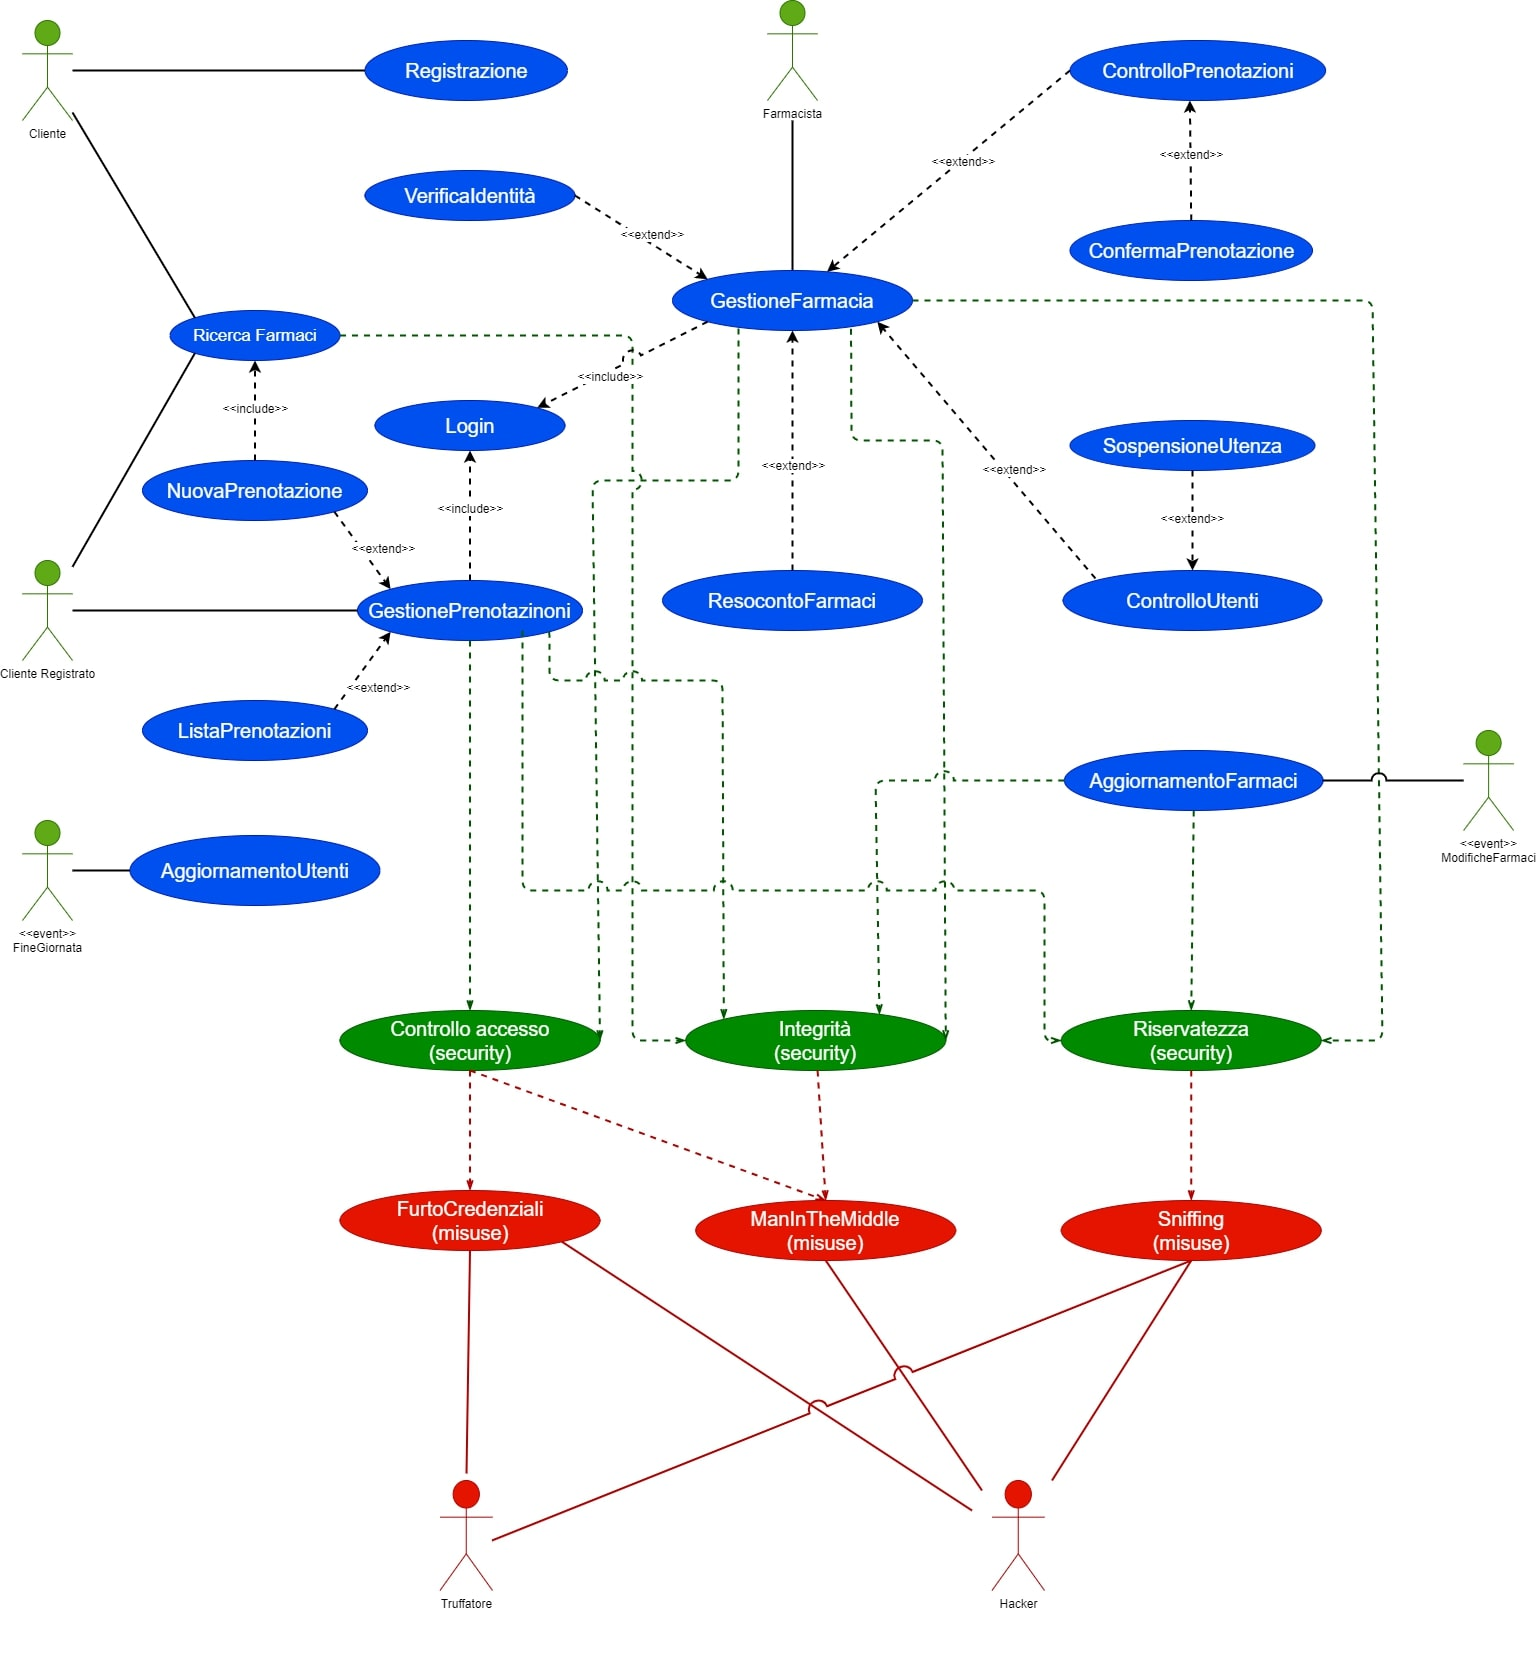
\includegraphics[width=\textwidth]{SecurityCase.jpg}
  \end{center}
\end{figure}
\newpage


\subsubsection{Security Use Case \& Misuse Case Scenari}
\hfill

\begin{tabular} {|P{4cm}|P{13cm}|}
\hline
  \textbf{Titolo} & Riservatezza\\
\hline
  \textbf{Descrizione} & I dati non sono accessibili da chi non ne ha i permessi\\
\hline
  \textbf{Misuse case} & Sniffing\\
\hline
  \textbf{Relazioni} &\\
\hline
  \textbf{Precondizioni} & L'attaccante ha i mezzi per intercettare i messaggi del sistema\\
\hline
  \textbf{Postcondizioni} & Il sistema impedisce all'attaccante di decifrare (in tempi utili) i messaggi intercettati\\
\hline
  \textbf{Scenario principale} & 1. Il Sistema protegge i messaggi \\ 2. L'attaccante riesce ad intercettare un messaggio \\ 3. L'attaccante prova a decifrare i messaggi, ma non riesce a trovare un modo per farlo abbastanza velocemente\\
\hline
  \textbf{Scenari di un attacco avvenuto con successo} & 1. Il Sistema protegge i messaggi \\ 2. L'attaccante riesce ad intercettare un messaggio \\ 3. L'attaccante riesce a decifrare i messaggi e a leggerne il contenuto, ma solamente per una sessione di un utente\\
\hline
\end{tabular}

\hfill
\break

\begin{tabular} {|P{4cm}|P{13cm}|}
\hline
\textbf{Titolo} & Integrità\\
\hline
  \textbf{Descrizione} & Integrità dei dati del sistema\\
\hline
  \textbf{Misuse case} & ManInTheMiddle\\
\hline
  \textbf{Relazioni} &\\
\hline
  \textbf{Precondizioni} & 1. L'attaccante ha i mezzi per intercettare i messaggi del sistema \\ 2. L'attaccante ha i mezzi per modificare i messaggi \\ 3. L'attaccante ha i mezzi per spedire il messaggio modificato al destinatario\\
\hline
  \textbf{Postcondizioni} & Il sistema rileva il messaggio contraffatto\\
\hline
  \textbf{Scenario principale} & 1. Il Sistema protegge i messaggi \\ 2. L'attaccante riesce ad intercettare un messaggio e lo modifica \\ 3. Il sistema si accorge del messaggio contraffatto e lo segna nei log\\
\hline
  \textbf{Scenari di un attacco avvenuto con successo} & 1. Il Sistema protegge i messaggi \\ 2. L'attaccante riesce ad intercettare un messaggio e lo modifica \\ 3. Il sistema accetta il messaggio e agisce di conseguenza, segnando il messaggio nei log\\
\hline
\end{tabular}
\\

\begin{tabular} {|P{4cm}|P{13cm}|}
\hline
  \textbf{Titolo} & ControlloAccessi\\
\hline
  \textbf{Descrizione} & L'accesso alle funzionalità del sistema deve essere controllato\\
\hline
  \textbf{Misuse case} & FurtoCredenziali, ManInTheMiddle\\
\hline
  \textbf{Relazioni} &\\
\hline
  \textbf{Precondizioni} & L'attaccante ha i mezzi per carpire in tutto o in parte le credenziali di accesso di un cliente o di un farmacista\\
\hline
  \textbf{Postcondizioni} & Il sistema blocca l'accesso non autorizzato e notifica il tentativo di accesso\\
\hline
  \textbf{Scenario principale} & 1. L'attaccante tenta di accedere al servizio spacciandosi per un utente legittimo, di cui conosce le credenziali solo in parte (ad esempio mediante attacco con dizionario) \\ 2. Il sistema non riconosce le credenziali, restituendo un errore \\ 3. In seguito ad un numero fissato di tentativi falliti, il sistema blocca temporaneamente l'accesso a quell'utente e notifica l'anomalia a chi di dovere\\
\hline
  \textbf{Scenari di un attacco avvenuto con successo} & 1. L'attaccante riesce a carpire le credenziali di accesso complete di un utente in un qualsiasi modo \\ 2. Il sistema riconosce la correttezza delle credenziali, e fornisce l'accesso al soggetto malevolo 3. L'attaccante ha libero accesso al sistema, con privilegi diversi in base al tipo di utente\\
\hline
\end{tabular}
\\

\subsubsection{Requisiti di Protezione dei Dati}

Sussistono inoltre i seguenti requisiti inerenti alla protezione dei dati: 
\begin{enumerate}
 \item I dati salvati devono essere protetti da un attaccante che abbia accesso al sistema, prendendo misure
di sicurezza fisica, eventualmente cifrando i dati. 
 \item I dati inviati tra le parti remote devono essere protetti, utilizzando la cifratura dei
dati. 
 \item Tutte le azioni avvenute sul sistema devono essere tracciate
tramite un sistema di log. 
\end{enumerate}

\raggedright{La visione e l'analisi dei log verrà gestita
con un editor di testo esterno, accessibile solo al personale
autorizzato.}
\hfill \break

\begin{tabular} {|P{3cm}|P{10cm}|P{3cm}|}
\hline
  \textbf{ID} & \textbf{Requisiti} & \textbf{Tipo}\\
\hline
  R16F & Implementazione di un sistema di log per tracciare tutti i messaggi tra i client e i server, inclusi gli accessi, le richieste di prenotazione, di conferma, di sospensione e di invio e ricezione di dati & Funzionale\\
\hline
  R9NF & I dati salvati devono essere protetti da un attaccante che abbia accesso al sistema, prendendo misure di sicurezza fisica, eventualmente cifrando i dati & Non Funzionale\\
\hline
  R10NF & I dati inviati tra le parti remote devono essere protetti, utilizzando la cifratura dei dati & Non Funzionale\\
\hline
\end{tabular}
